\section{Wahrscheinlichkeit}
\subsection{Wahrscheinlichkeitsdichte}
Die Fläche zwischen einem Punkt $a$ und $b$ zeigt die Wahrscheinlichkeit an. Nicht der Wert von der Wahrscheinlichkeitsdichtefunktion ist somit relevant, sondern die Fläche unter ihrm Graphen. Die Wahrscheinlichkeitsdichte muss daher auch den Flächeninhalt $1$ haben. 
\[
\int_{-\infty}^{\infty}\varphi(x)dx = 1
\]
Siehe \textbf{Beispiel} Kapitel \ref{wdichte}.

\subsection{Verteilungsfunktion}\script{83}
Die Verteilungsfunktion $F$ gibt an, mit welcher Wahrscheinlichkeit das Ergebnis des Zufallsexperiments kleiner oder gleich eines bestimmten Wertes ist. Dafür werden alle Ergebnisse bis zu diesem Wert summiert. 
\[
\varphi(x) = F'(x) \xRightarrow[]{} \int_{-\infty}^{x}\varphi(\zeta)d\zeta = F_x(x)
\]
$F$ ist die Stammfunktion von der Wahrscheinlichkeitsdichte $\varphi$.

\subsubsection{Gleichverteilung}\script{101}
Gleichverteilung liegt zB vor wenn Zufallszahlen  in einem Intervall von $[a, b]$ gleichverteilt sind. Jede Zahl sollte gleich Wahrscheinlich vorkommen. Der Erwartungswert kann einfach durch $E(X) = \frac{a + b}{2}$ bestimmt werden. für Varianz gilt $\var(x) = \frac{(b-a)^2}{12}$
\[
\varphi(x) = \begin{cases}
	0 & x < a \\
	\frac{1}{b-a} & x \in [a,b] \\
	0 & x > b
\end{cases}
\]

\subsubsection{Exponentialverteilung}\script{104}
Gedächnislose Prozesse wie Radioaktiver Zerfall, Bauteile ohne Ermüdungserscheinungen oder Warteschlangen.
\[\varphi(x) = \begin{cases*}
	ae^{-ax} \qquad x \geq 0 \\
	0 \qquad \text{sonst}
\end{cases*}\]
Parameter a bestimmt den \textit{Mean Time between Failure} oder Erwartungswert: 
\[E(X) = \frac{1}{a} \qquad \var(x) = \frac{1}{a^2}\]

\noindent Die \textbf{Halbwertszeit} ist auch der Median:
\[ \med(T) = \frac{1}{a}\ln2 \] 

\subsubsection{Normalverteilung}\script{109}
Summe vieler kleiner Einflüsse wie Messwerte oder wiederholte Experimente. Zwei Drittel aller Werte liegen innerhalb einer Standardabweichung $\sigma$ um den Erwartungswert $\mu$. Diese Verteilung wird verwendet, wenn $P$ irgendwo in der mitte liegt, für seltene (kleine $P$) kann die Piossonverteilung verwendet werden.
\[
\varphi(x) = \frac{1}{\sigma\sqrt{2\pi}}e^{-\frac{(x-\mu)^2}{2\sigma^2}}
\]
\noindent Die Varianz ist zudem gegeben durch die Wendestellen bei $\mu \pm \sigma \rightarrow \var(x) = E(X^2) - E(X)^2 = \sigma^2E\left(\frac{(x - \mu)^2}{\sigma^2}\right)$

\begin{center}
	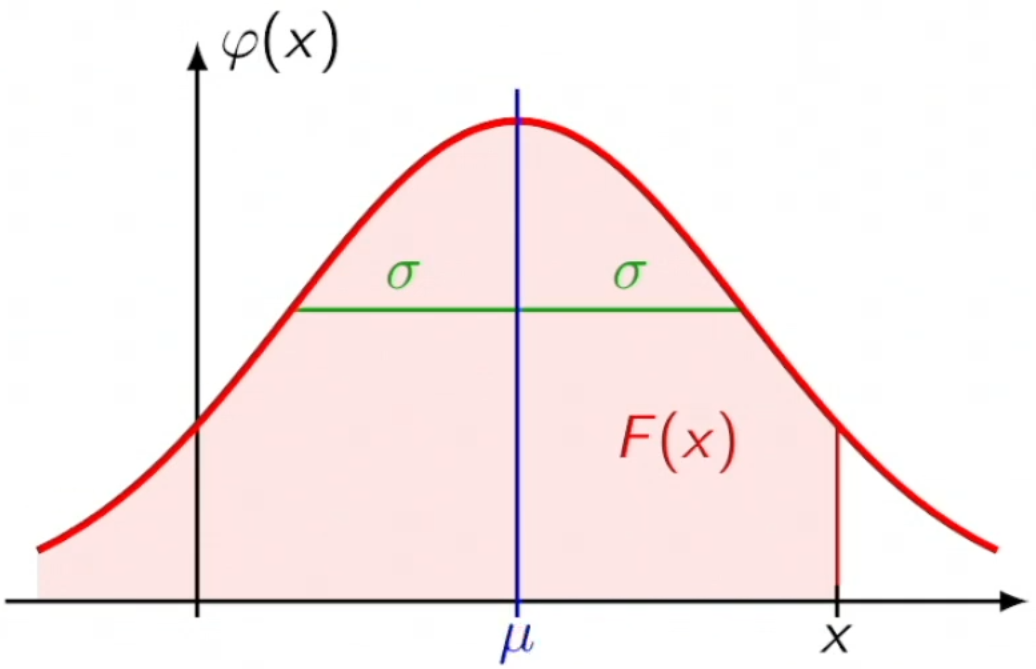
\includegraphics[width=0.4\columnwidth]{Images/normalverteilung}
\end{center}

\noindent Wenn die Normalverteilung Standardisiert wurde, kann die Tabelle verwendet werden. $\Phi(-x) = 1 - \Phi(x)$:\\
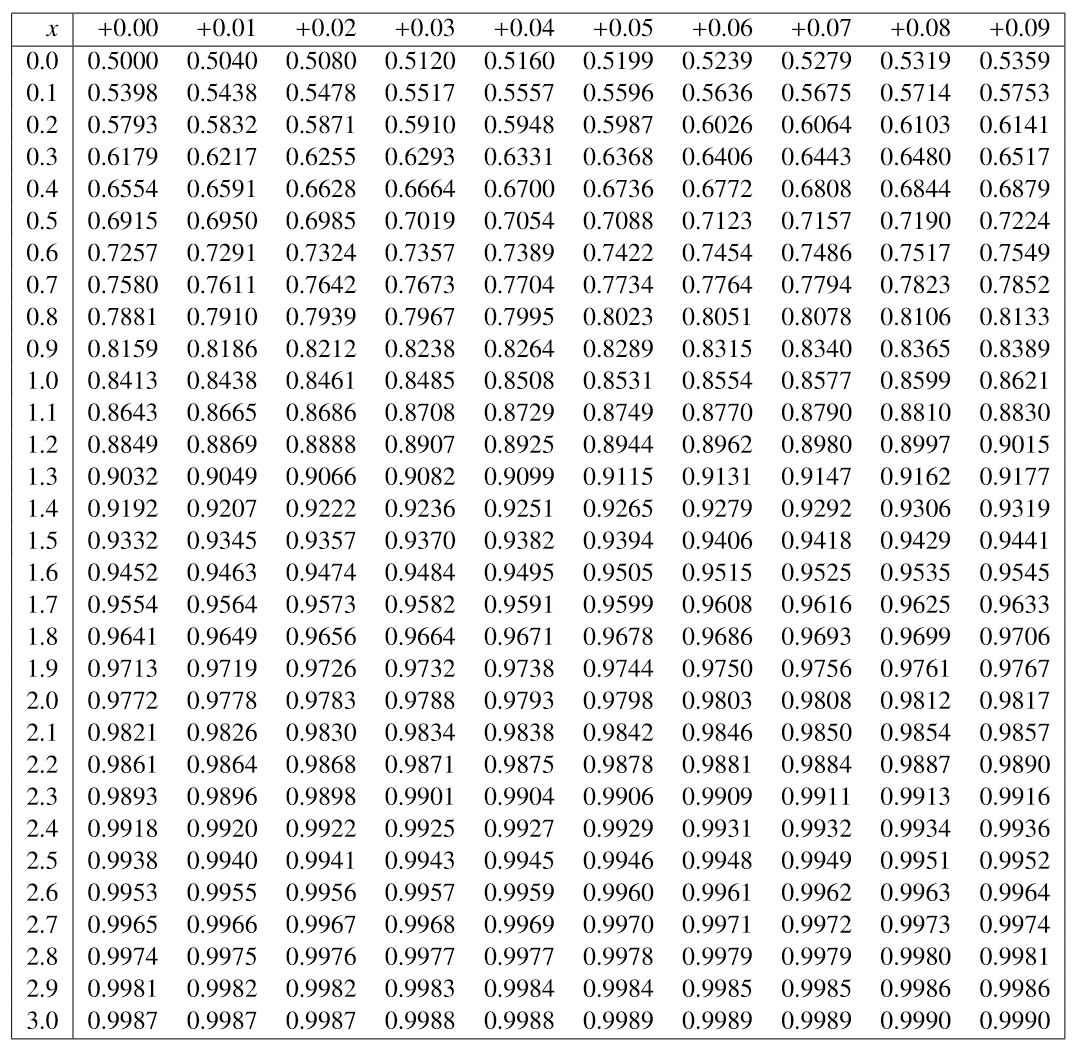
\includegraphics[width=\columnwidth]{Images/standard-normalverteilung}

\subsubsection{Poissonverteilung}\script{136}
Gedächnislose Prozesse $T_i$ mit gleichem $a$. Wobei $k$ die Anzahl der Prozesse und $\lambda = al$ mit $l$ der Länge auf dem Intervall ist. $\lambda$ kann auch eine Rate sein. \textbf{Achtung:} Dies sollte nur verwendet werden, wenn $n$ gross und $P$ selten ist.
\[
P_k(\lambda) = e^{-\lambda}\frac{\lambda^k}{k!}
\]
\noindent\textbf{Beispiel:} Siehe Kapitel \ref{approx_poission}

\subsection{Binomialverteilung}
Zufallsexperiment mit zwei möglichen Ausgängen $A$ oder $\overline{A}$ zB Lotto, Wahrscheinlichkeit $p = P(A)$. $X$ = Anzahl Eintreten von $A$ in $n$ unabhängigen Durchführungen. Der Erwartungswert kann auch durch $E(X) = np$ und die Varianz $\var(X) = np(1 - p)$ berechnet werden.
\[
P(X = k) = \underbrace{\begin{pmatrix}	n \\ k \end{pmatrix}}_{\text{Anzahl Auswahl}}\cdot \underbrace{p^k}_{\text{Eintreten von A}}\cdot\underbrace{(1-p)^{n-k}}_{\text{Eintreten von }\overline{A
}}
\]
\noindent\textbf{Beipsiel:} Wie gross ist die Wahrscheinlichkeit, dass bei 10 Würfen einees fairen Würfels 7 mal die 5 kommt. Das Einzelereignis ist $p = P(\text{Augenzahl } 5) = \frac{1}{6}$
\[
P (X = 7) = \begin{pmatrix}	10 \\ 7 \end{pmatrix} \frac{1}{6^7}\begin{pmatrix}	5 \\ 6 \end{pmatrix}^3 = 0.000248
\]
\subsubsection{Approximation Normalverteilung}
Für grosse $n$ und eher grosse $p$ kann die Binomialverteilung auch mit der Standard- Normalverteilung approximiert werden. Damit werden $\mu = np$ und $\sigma = \sqrt{np(1-p)}$ standardisierte. \textbf{Achtung:} für die Grenzen immer $\pm 0.5$ addieren, um Rundungsfehler zu minimieren.
\begin{align*}
	P(X \leq k) &\approx \Phi(\frac{k + 0.5 - \mu}{\sigma}) \\
	P(l < X \leq k) &\approx \Phi(\frac{k + 0.5 - \mu}{\sigma})  - \Phi(\frac{k - 0.5 - \mu}{\sigma}) \\
\end{align*}
\noindent\textbf{Beispiel:} Siehe Kapitel \ref{approx_normal}

\subsubsection{Approximation Poissonverteilung}
Für grosse $n$ und eher kleine $p$ wird die Binomialverteilung besser mit der Poissonverteilung approximiert. $\lambda = np$
\[
P_\lambda(k) = e^{-\lambda}\frac{\lambda^k}{k!}
\]
\noindent\textbf{Beispiel:} Siehe Kapitel \ref{approx_poission}

\subsection{Hypergeometrische Verteilung}\script{135}
Von $N$ Objekten sind $M$ markiert. Daraus werden $n$ Objekte zufällig ausgewählt.

\begin{center}
	\begin{minipage}{0.20\textwidth}
		\begin{center}
			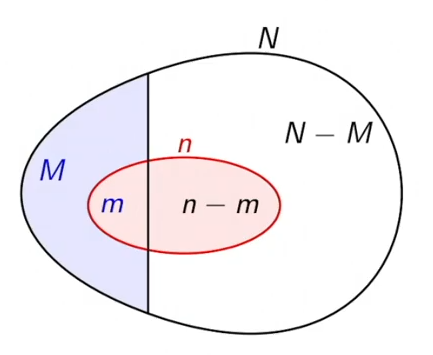
\includegraphics[width=\linewidth,keepaspectratio=true]{Images/hypergem-verteilung}\\
		\end{center}
	\end{minipage}%%% to prevent a space
	\begin{minipage}{0.3\textwidth}
	\[
	P(X=m) = \frac{\begin{pmatrix}	M \\ m\end{pmatrix}\begin{pmatrix}	N-M \\ n-m\end{pmatrix}}{\begin{pmatrix} N \\ n\end{pmatrix}}
	\]
	\end{minipage}
\end{center}


\subsubsection{Gamma-Verteilung}
Die Gamma-Funktion kann zB for die Warteschlangetheorie oder Versicherungsmathematik verwendet. Sie ist mit Parametern $v=\frac{n}{2}$ und $\alpha=\frac{1}{2}$ die verallgemeinerung der $\chi^2$-Verteilung 
\[
\gamma_{\alpha,v}(x) = \frac{1}{\Gamma(v)\alpha^vx^{v-1}e^{\alpha x}}
\]

\subsection{$\chi^2$-Verteilung}\script{126}
Siehe \ref{chi-verteilung}